% !Mode::"TeX:UTF-8"
\documentclass[UTF8]{article}   %this [UTF8] is very important
\usepackage{ctex}               %中文支持
\usepackage{fancyhdr}           %页眉页脚
\usepackage{geometry}           %调整页边距
\geometry{a4paper,left=2cm,right=2cm}
\usepackage{underscore}         %支持下划线作为文本输入
\usepackage{graphicx}           %支持图片插入
\usepackage{float}
\usepackage{amssymb}            %支持数学符号
\usepackage{xlop}               %支持竖式除法的排版
\usepackage{booktabs}           %支持表格的线
\usepackage{caption}            %设置字体
\usepackage{listings}           %支持代码
\usepackage{varwidth}           %支持图片顶部对齐
\usepackage{amsmath}            %支持多行公式的数学环境
\usepackage{epstopdf}           %支持pdfLatex下用eps
\usepackage{multirow}           %支持合并单元格
\usepackage{longtable}          %支持长表格
\usepackage{appendix}
\usepackage{colortbl}           %支持彩色表格
\usepackage{color}

\chead{\thesection}
\cfoot{\thepage}
\author{朱德森}
\title{GDB-调试点}
\begin{document}
\songti
\linespread{1.3}
\maketitle
\tableofcontents
\newpage

\section{背景}
在进行程序的调试时,
经常需要反复运行程序至问题所在,
而有时需要等待大量时间运行至问题处,
若不能成功定位到问题,
就需要重新运行,
消耗大量不必要的时间。

GDB 的调试点针对该问题提供了解决方案,
在调试过程中即使没能定位到问题,
也只需要花费一次时间运行至问题处。

GDB 调试点 (checkpoint) 的原理是复制进程的方式,
当程序运行到问题点处时,
通过 checkpoint 命令将当前调试进程复制一份。
那么当第一个进程执行到问题点之后时,
可以切换至复制出的进程,
此时复制出的进程依然停留在问题点处,
可以再一次进行调试,
而不需要将程序重头运行一遍。

\section{常用命令}
\begin{itemize}
    \item checkpoint              : 生成新的调试点
    \item restart [num]           : 跳转到调试点 [num]
    \item delete checkpoint [num] : 删除调试点 [num]
    \item info checkpoint         : 查看当前所有调试点信息
\end{itemize}

\section{举例使用}
下面提供了一个工程例子进行说明,
如图 \ref{fig:main} 所示,

本段代码主要是模拟一个百分数的累加,
也可以认为是程序进度的一个指示。
为了调试,在 AddPercent 函数中人为地引入了一个 bug,
导致在主程序中百分比的累加出现不连续,
下面将利用这段程序来演示 checkpoint 调试点的使用。

\begin{figure}[H]
\begin{center}
    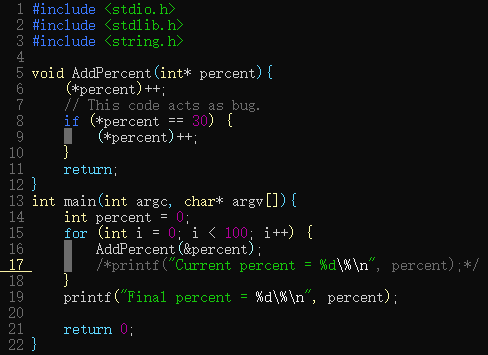
\includegraphics[width=0.8\textwidth]{./pic/main}
\end{center}
\caption{代码例子}
\label{fig:main}
\end{figure}

\begin{figure}[H]
\begin{center}
    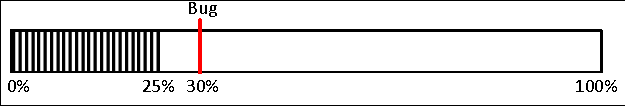
\includegraphics[width=0.8\textwidth]{./pic/NoCheckpoint}
\end{center}
\caption{代码例子}
\label{fig:main}
\end{figure}

\begin{figure}[H]
\begin{center}
    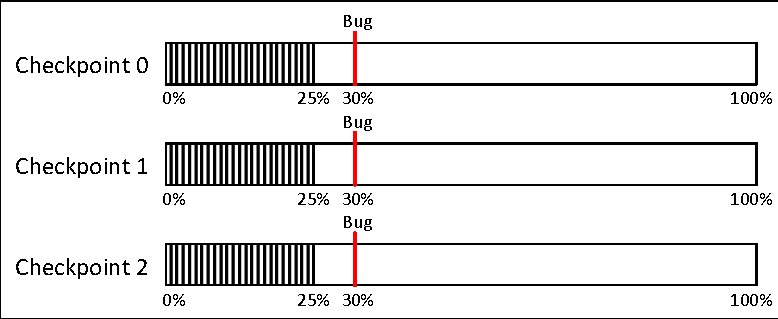
\includegraphics[width=0.8\textwidth]{./pic/CopyCheckpoint}
\end{center}
\caption{代码例子}
\label{fig:main}
\end{figure}

\begin{figure}[H]
\begin{center}
    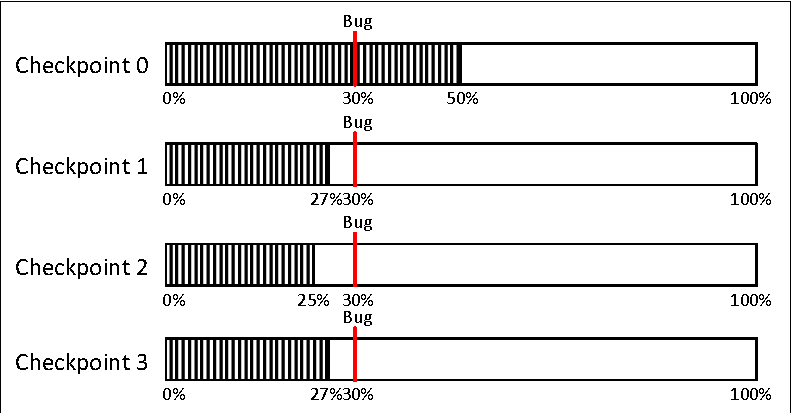
\includegraphics[width=0.8\textwidth]{./pic/RunAndCopyCheckpoint}
\end{center}
\caption{代码例子}
\label{fig:main}
\end{figure}

\section{参考资料}
\begin{itemize}
    \item gdb使用小技巧-保存调试点现场 (https://www.cnblogs.com/qinghaowusu/p/13994017.html)
\end{itemize}




\end{document}
